\chapter{An Autonomous Robotic Team for the Rapid Characterization of Novel Environments}

In this chapter, we present preliminary results from our autonomous robotic team. First we detail the development of a real time processing and georectification pipeline for the hyperspectral images collected by our drone. This is vital to enable real time application of the robotic team in realistic field settings. Next we discuss results of apply machine learning to directly model concentrations of of chemicals-of-concern form the captured reflectance spectra. Finally, we provide discuss the application of unsupervised methods including the SOM and GTM developed in chapter 3 to enable a physics-based unsupervised learning framework for the identification of novel constituents. Associated code are made freely accessible at \url{https://github.com/john-waczak/RobotTeam.jl}

\section{Rapid Processing and Georectification of Hyperspectral Data Cubes}

The increased spectral resolution of HSI systems poses unique challenges to their adoption for real time applications primarily stemming from the considerable size of generated data files. Current data collection workflows see researchers first perform the aerial survey (data collection) and then transfer data to ground based computers for post processing. This workflow is well established in the remote sensing community where, as an example, compressed raw imagery from Sentinel-2 are transferred to the ground and then subsequently post processed into their final L1C (top of atmosphere) and L2A (bottom of atmosphere) data products \cite{sentinel-processing, sentinel-products}. Drone based applications often operate in a similar manner: images or video are collected by a survey and then post-processed and analyzed with software such as Open Drone Map to produce the desired data products (tile mosaics, 3d reconstructions, etc.) \cite{copernicus-odm}. For an HSI platform to function in real time, three key tasks are critical:
\begin{enumerate}
\item \textbf{FileIO}: Raw imagery need to be quickly read by the on-board processing computer.
\item \textbf{Post-processing}: Raw imagery need to be rapidly converted to the chosen data product (typically, Reflectance), and importantly, must be georeferenced so that each image pixel can be located on the ground.
\item \textbf{Ground Transfer}: Sufficient wireless communication capabilities must be avaiable to transmit the final data products.
\end{enumerate}
The first can be readily accomplished by means of light-weight, high volume solid state drives incorporated into the imaging system. To address the second, we need both sufficient compute and optimized processing software. Finally, ground transfer of final post-processed data products can be accomplished in a variety of ways. As we rarely need the full hyper-spectral datacube immediately, we can generate the desired data products on-board (NDVI for example) and transfer only the relevant information to a ground station.To enable this workflow, our drone is outfitted with two additional components critical for this application. The first is a pair of light-weight processing computers (Intel NUCs).  One is attached directly to the imager and manages data acquisition and saving of raw data files. The second NUC is mounted above the payload and serves as the onboard data processing unit. As illustrated in Figure \ref{fig:drone-components}, we also equip the drone with an upward facing irradiance spectrometer outfitted with a cosine corrector (to integrate over a half-sphere of solid angle).
\begin{figure}[!hbt]
  \centering
  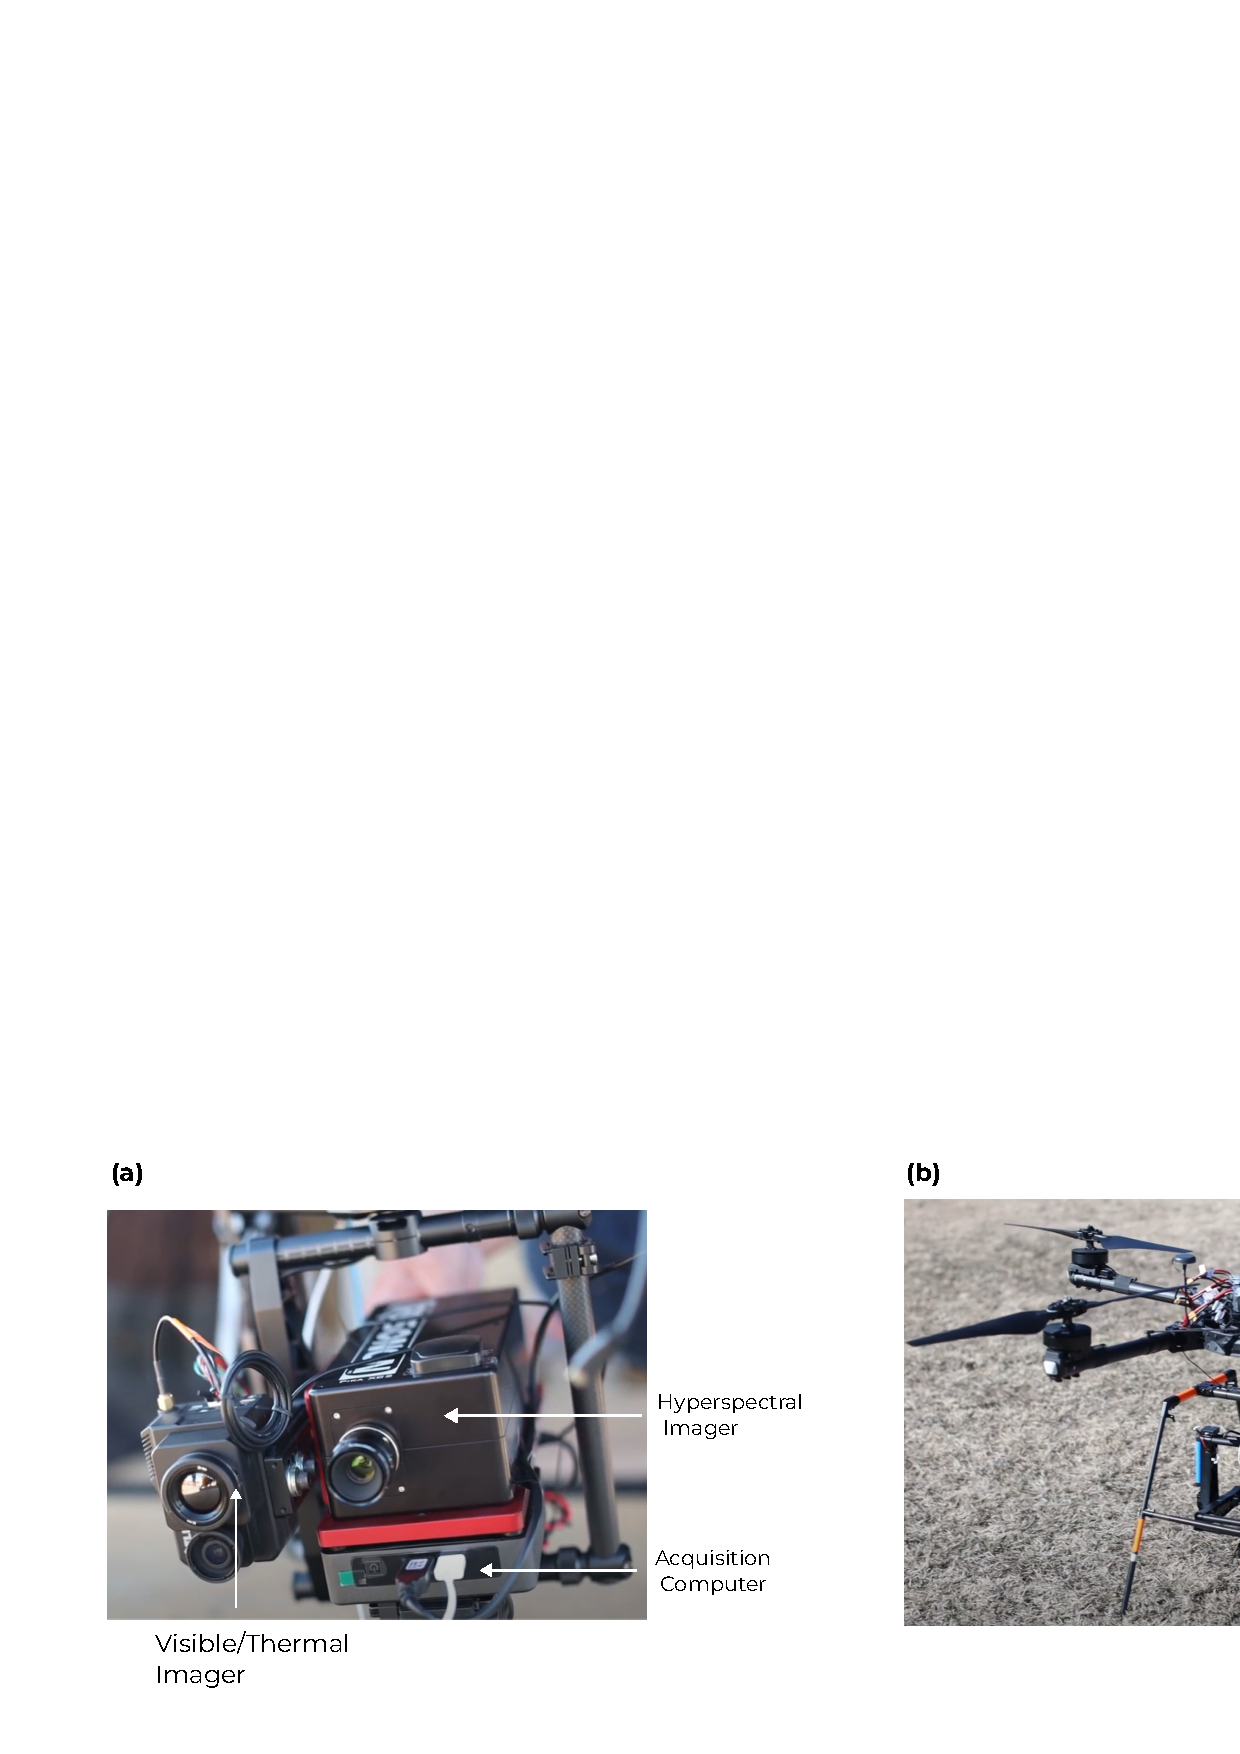
\includegraphics[width=0.85\columnwidth]{robot-team/assets/annotated-drone.pdf}
  \caption{Components of the Autonomous Drone HSI platform.}
  \label{fig:drone-components}
\end{figure}
This spectrometer captures the \textit{downwelling} irradiance spectrum which is necessary to enable conversion from radiance units to the desired reflectance spectra. To this end we present a procedure based on the methods described in \cite{muller-georeferencing, GeorectivicationBaumker, GeorectificationMostafa} for the rapid processing and georeferencing of imagery captured by a pushbroom HSI mounted on an autonomous drone. The processing steps are as follows:
\begin{enumerate}
\item Raw imagery are continuously captured by the hyperspectral imager (Radiance) and stored in binary ENVI format.
\item The processing computer reads ENVI files into tensors as they become available.
\item Associated flight data (GPS and IMU) are read.
\item Flight data are interpolated to match the sample times for each scan-line.
\item The HSI is georeferenced to obtain coordinates (lat,lon) for each pixel.
\item The georeferenced HSI is then resampled to a regular grid.
\item The downwelling irradiance spectrum associated with the HSI is read.
\item The downwelling spectrum is interpolated to match the wavelength bins of the HSI
\item The HSI is converted o Reflectance under the assumption of a Lambertian surface (perfectly diffuse).
\item Any desired derived $\lambda$-metrics (NDVI, etc...) are computed.
\item Data products are selected and the result is transferred to the ground station.
\end{enumerate}

\begin{figure}[h]
  \centering
  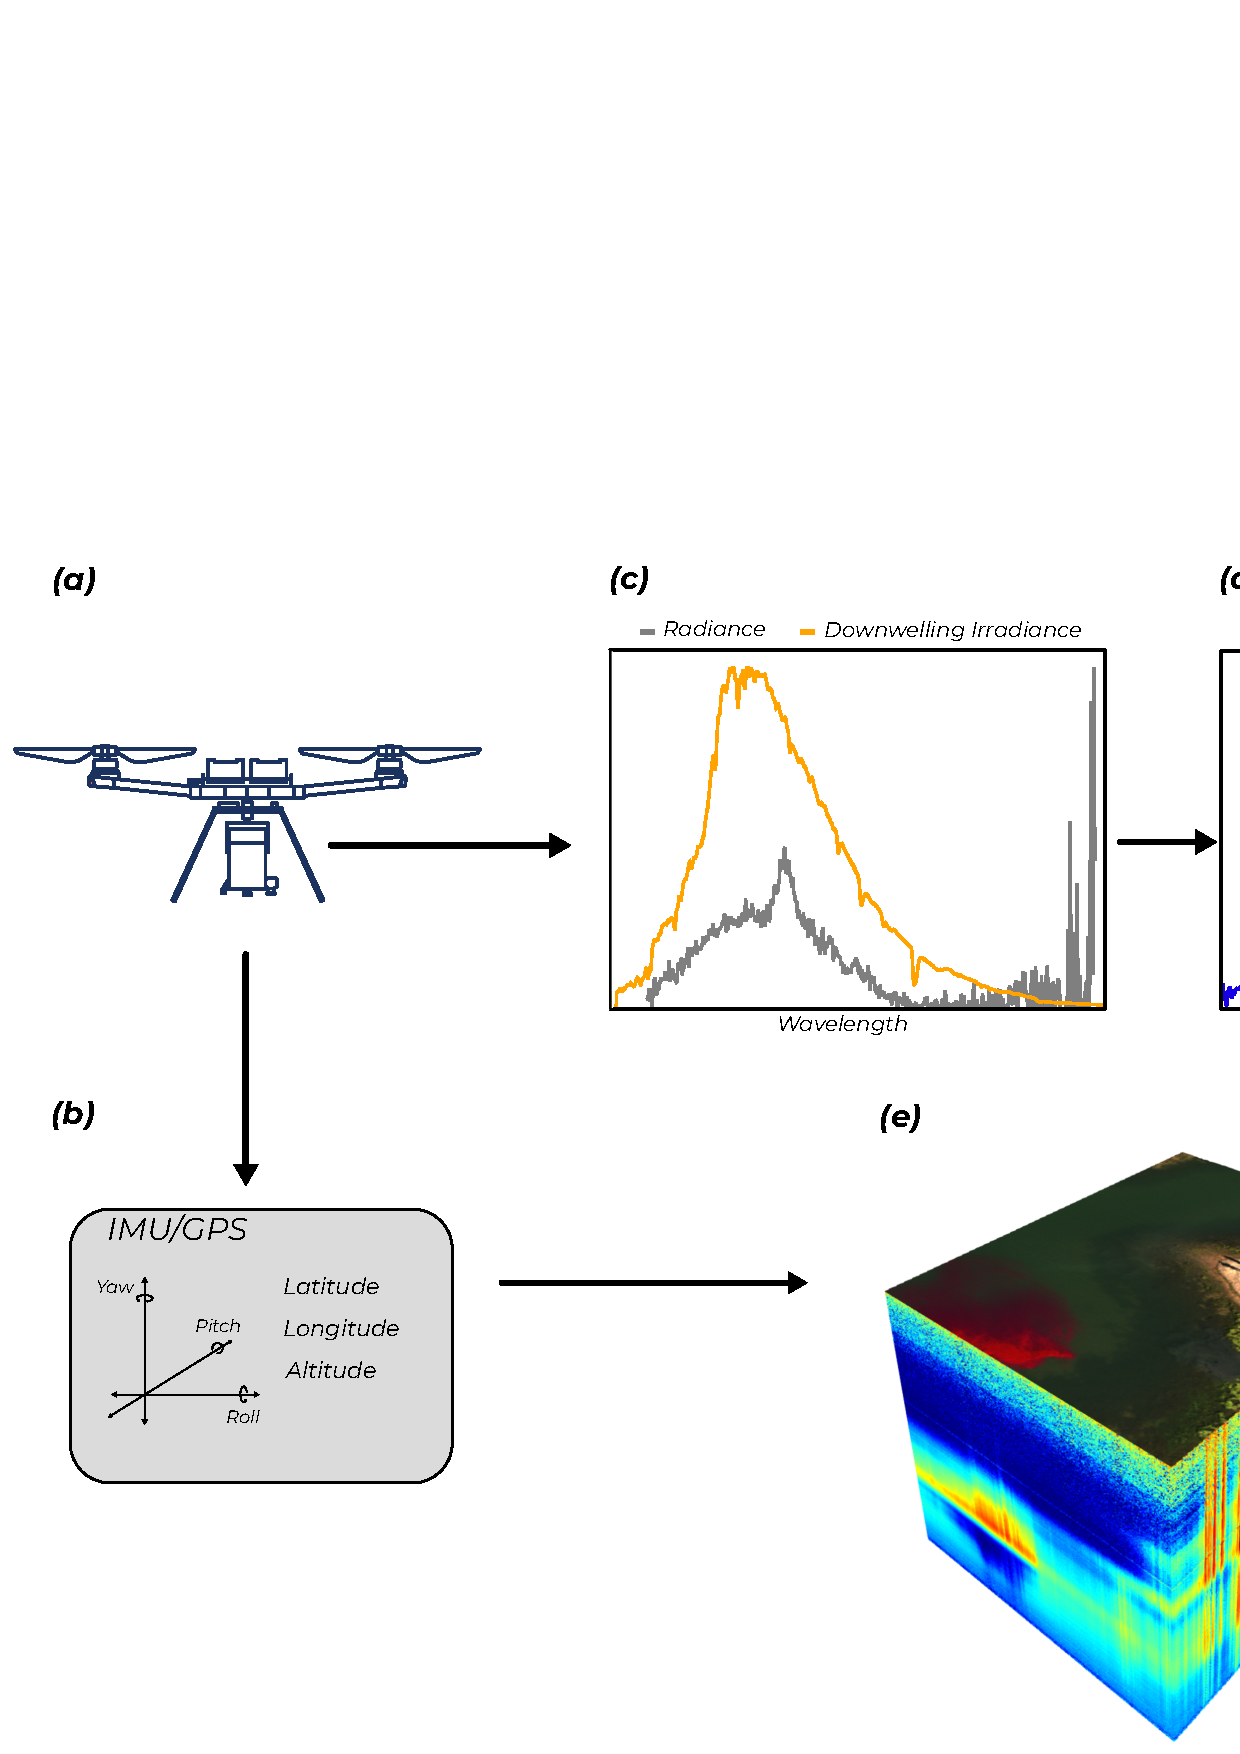
\includegraphics[width=0.85\columnwidth]{robot-team/georectification/pipeline-figure.pdf}
  \caption{Visual representation of the processing pipeline}
  \label{fig:annotated-hsi}
\end{figure}


\subsection{Georeferencing and Resampling}

The hyperspectral imager used on our autonomous drone is different from a typical camera; instead of capturing an image by collecting light onto an array of sensors, our HSI is configured as a pushbroom imager. In this configuration, a single scanline of pixels is captured by the sensor and an image is formed as the drone flies along its route. This poses an interesting challenge for georeferencing as each individual scanline needs to be transformed independently. If the drone's path winds and turns, each subsequent scanline will be stretched and rotated independently based on the relative orientation of the drone to the ground at the time of capture. This sampling geometry as well as the relevant orientation angles are illustrated in Figure \ref{fig:georectification}.

\begin{figure}[h]
  \centering
  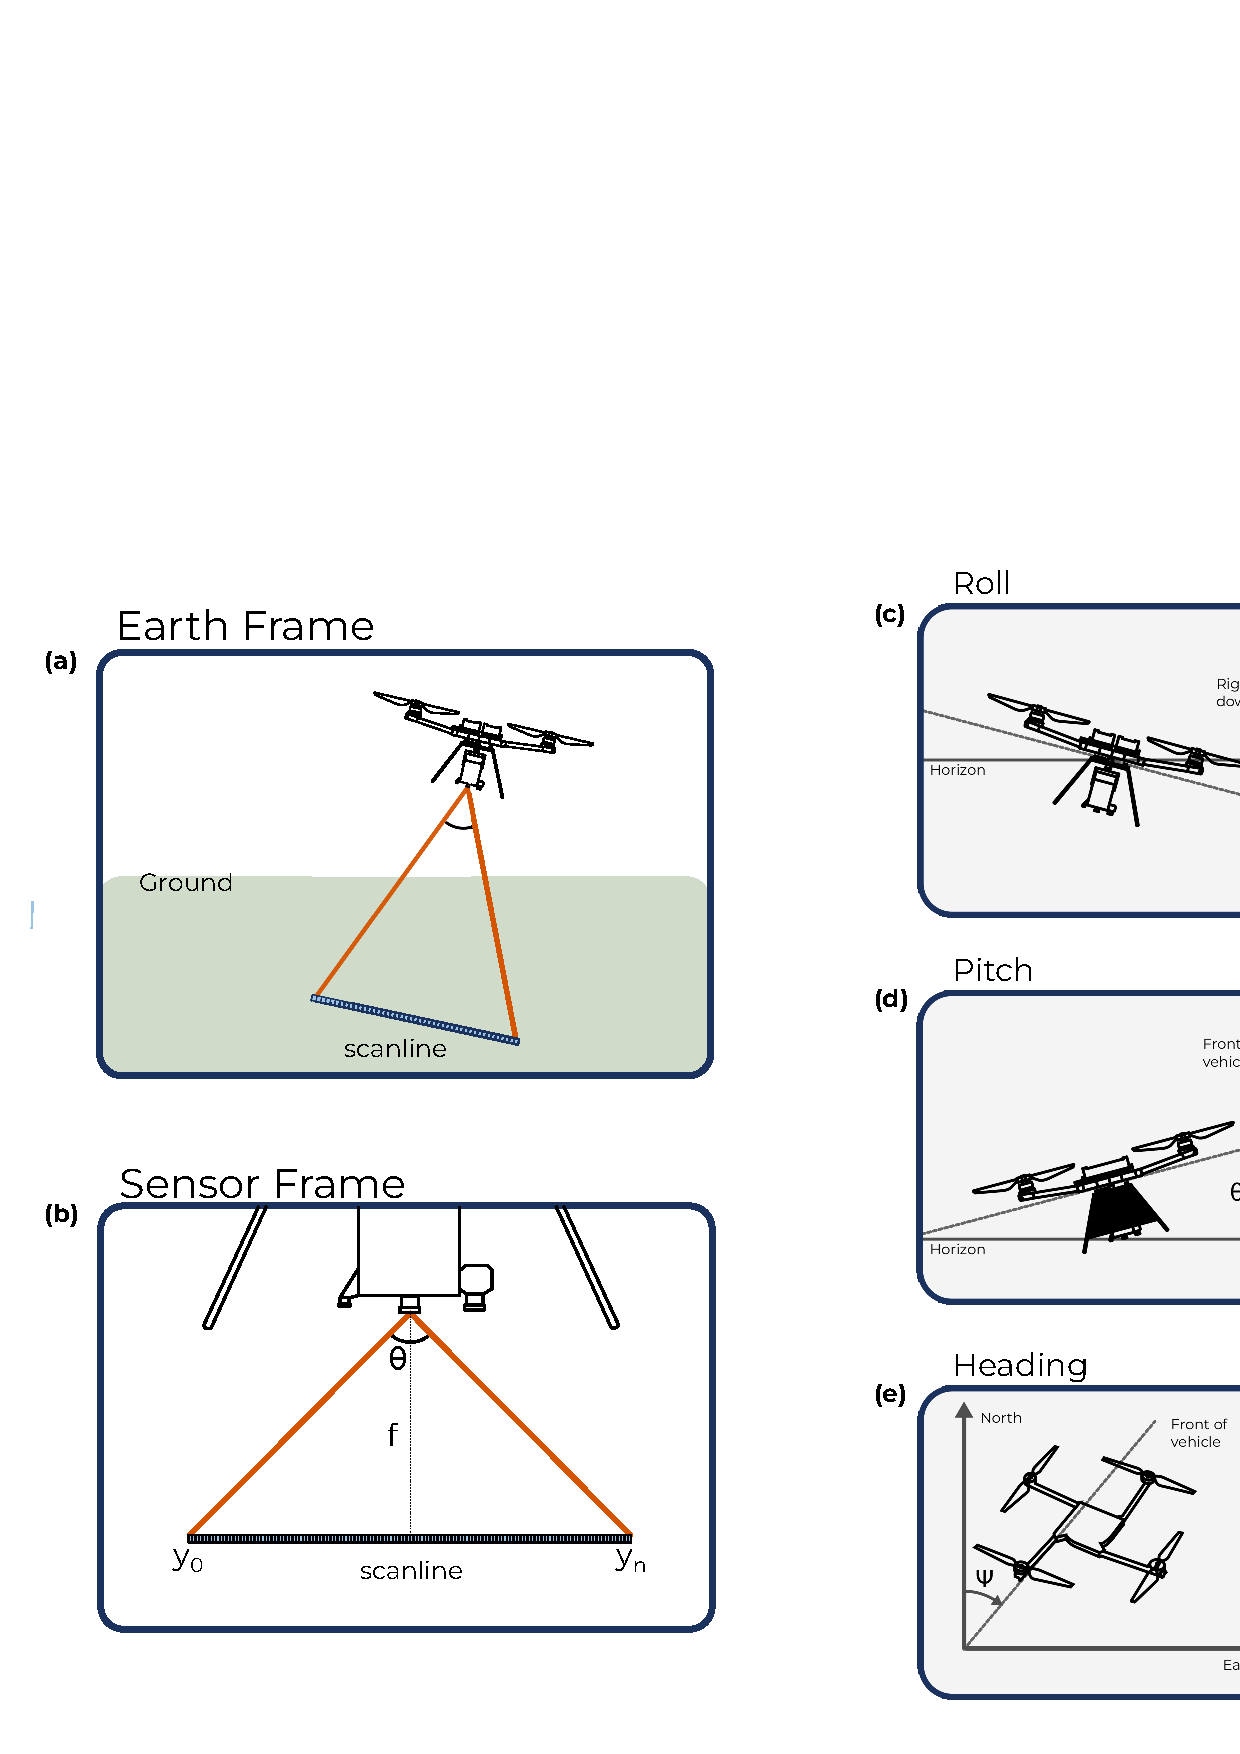
\includegraphics[width=0.85\columnwidth]{robot-team/assets/georectification.pdf}
  \caption{Visual representation of scan-line geometry for the drone based hyperspectral imaging platform.}
  \label{fig:georectification}
\end{figure}

The GPS and IMU on the hyperspectral imager capture the location $(\lambda, \Phi, z)^T$  (longitude, latitude, altitude) of our drone as well it's orientation defined by the angles $\phi$, $\theta$, and  $\psi$ (roll, pitch, and heading) at the time of capture of each scanline. To georeference each pixel, we therefore must transform its position from the frame of the sensor (measured in pixels relative to the HSI) first to the frame of the IMU used to measure the orientation, then to the navigation frame (east, north, up), and finally to the ground frame. Let us define the \textit{sensor} frame so that the scanline falls upon the y axis. As each scanline must be transformed independently, we can assign it an x-coordinate of $0$ pixels. Lastly, if the viewing angle of the HSI is $\theta_{\text{view}}$, then the coordinates of the i\textsuperscript{th} pixel, $\mathbf{r}_i^{\text{sensor}}$, in the sensor frame are defined as in panel (b) of Figure \ref{fig:georectification}, namely
\begin{equation}
  \mathbf{r}_i^{\text{sensor}} = \left(0, y_i, f \right)^T
\end{equation}
where $y_i\in \left\{-\frac{(N-1)}{2},...,\frac{N-1}{2}\right\}$ and $f=\frac{(N-1)/2}{\tan(\theta_{\text{view}}/2)}$ for $N$-total pixels per scanline. To align the sensor frame with the axes of the IMU, we apply a sequence of rotation matrices defined using the measured orientation angles (panels (c), (d), and (e) of Figure \ref{fig:georectification}), which we call
\begin{equation}
  \begin{aligned}
    &R_{\text{sensor}}^{\text{IMU}}(\phi,\theta,\psi) = \\
    &\begin{bmatrix}
    \cos(\psi)\cos(\theta) & \cos(\psi)\sin(\theta)\sin(\phi)-\sin(\psi)\cos(\phi) & \cos(\psi)\sin(\theta)\cos(\phi)+\sin(\psi)\sin(\phi) \\
    \sin(\psi)\cos(\theta) & \sin(\psi)\sin(\theta)\sin(\phi)+\cos(\psi)\cos(\phi) & \sin(\psi)\sin(\theta)\cos(\phi)-\cos(\psi)\sin(\phi) \\
    -\sin(\theta) & \cos(\theta)\sin(\phi) & \cos(\theta)\cos(\phi)
     \end{bmatrix}
  \end{aligned}
\end{equation}

Next, we apply an orthogonal transformation to transform from the IMU frame to the navigation frame of the drone. This is important as the axes of the IMU and the drone itself are not necessarily identical depending on how the IMU is oriented on the HSI. For us, this amounts to
\begin{equation}
  T_{\text{IMU}}^{\text{DRONE}} = \begin{bmatrix}
    0 & 1 & 0 \\
    1 & 0 & 0 \\
    0 & 0 & -1
    \end{bmatrix}
\end{equation}
At this stage, we have now transformed the pixel coordinates into the frame of the drone. Next using the similar triangles defined by the sensor and navigation frames (panels (a) and (b) of Figure \ref{fig:georectification}), we can rescale the coordinates into units of meters by introducing the scale factor
\begin{equation}
  s = \frac{z-z_{\text{ground}}}{f\cos(\theta)}.
\end{equation}
Finally, we translate the coordinates of each pixel using the position of the drone in the chosen coordinate system. As the geometric transformations are scaled to units of meters (by $s$), we apply a coordinate transformation $f$ to obtain the position of the drone with respect to a local coordinate system such as the Universal Transverse Mercator (UTM). Written all together, this takes the form
\begin{equation}
  \mathbf{r}_{i}^{\text{UTM}} =
  f_{\text{geo}}^{\text{UTM}}\begin{bmatrix}
    \lambda \\
    \Phi \\
    z_{\text{drone}}
  \end{bmatrix}_{\text{GPS}}^{\text{geo}} + sT_{\text{IMU}}^{\text{DRONE}}R_{\text{sensor}}^{\text{IMU}}(\theta, \phi, \psi)\begin{bmatrix}
    0 \\
    y_i \\
    f
  \end{bmatrix}^{\text{sensor}}
\end{equation}

For each image, the above transformation can be applied \textit{in parallel} across all scanlines to obtain the ground coordinates $\mathbf{r}_i=(x_i, y_i,z_i)^T$ of each pixel. To aid in further analysis and enable the generation of data products, it is often desirable to resample the georeferenced datacube to a regular grid. To accomplish this rapidly, we can define a bounding box by the extrema of the pixel coordinates. Then, for a desired resolution, say $\Delta x$ in meters, we truncate each pixels coordinates to the nearest $\Delta x$ and then average all pixels that have the same position.


\subsection{Reflectance Conversion}

Once we have georeferenced and resampled the hyperspectral datacube we can use the measured downwelling irradiance spectrum to convert the raw data from radiance to reflectance. This allows us to normalize for the incident light so that spectra captured under variable lighting conditions can be compared. First, the downwelling irraidance spectrum is loaded and interpolated to match the wavelengths of the spectral bins for our HSI. The reflectance at pixel $(i,j)$ and wavelength $\lambda_k)$ is then obtained by
\begin{equation}
  R_{ijk} = \frac{\pi L_{ijk}}{E_k}
\end{equation}
where $L_{ijk}$ denotes the original radiance pixel and $E_k$ denotes the downwelling irradiance at wavelength $\lambda_k$. This conversion makes the assumption that the surface can be treated as \textit{Lambertian}, that is, that the surface is perfectly diffuse and scatters light according to the cosine emission law which when integrated over a half sphere of solid angle introduces the factor of $\pi$.

\begin{figure}[h]
  \centering
  \includegraphics[width=0.85\columnwidth]{robot-team/georectification/hsi-infographic.pdf}
  \caption{Annotated view of a hyperspectral data cube showcasing sampled spectra for a variety of constituents.\label{fig:hsi-infographic}}
  \label{fig:annoted-hsi}
\end{figure}  

Figure \ref{fig:annotated-hsi} illustrates the reflectance spectra for a variety of constituents in a sample hyperspectral data cube. In panel (a) we show a typical downwelling irradiance spectrum. Panels (c)-(f) show a selection of reflectance spectra for open water, a rhodamine dye plume, algae near the shore, and dead grass. Panel (b) is a visual representation of the hyperspectral data cube with reflectance at each wavelength bin along the z axis and a pseudo color image showing the imaging scene on the top.


%%%%%%%%%%%%%%%%%%%%%%%%%%%%%%%%%%%%%%%%%%
\section{Timing Results}


\begin{table}[h]
  \centering
  \begin{tabular}{ |c|c| }
    \hline 
    \textbf{Number of scan lines}	& \textbf{Execution time (s)}\\
    \hline 
    371		&   2.060	\\
    725     &   4.227	\\
    1000    &   5.901  \\
    \hline 
  \end{tabular}
  \caption{Reflectance conversion time as a function of number of scanlines}
  \label{tab:reflectance-times}
\end{table}

\begin{figure}[!hbt]
  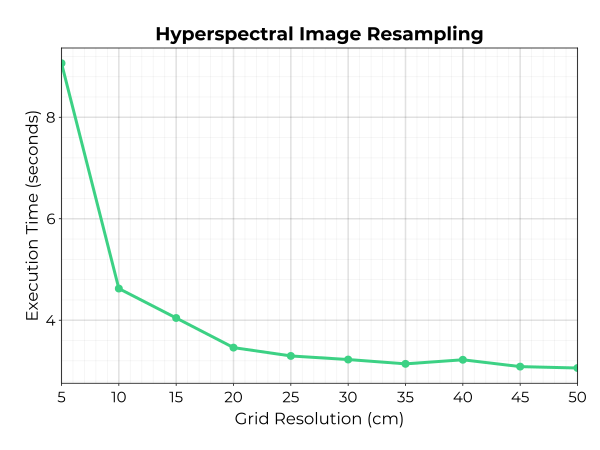
\includegraphics[width=0.85\columnwidth]{robot-team/georectification/regrid-timing.pdf}
  \caption{}
  \label{fig-regridding-timing}
\end{figure}



%%%%%%%%%%%%%%%%%%%%%%%%%%%%%%%%%%%%%%%%%%
\section{Discussion}



\section{Supervised Regression with Uncertainty Quantification}

\subsection{Hyperspectral Imaging and Remote Sensing}
paper creating new spectral index for wheat rust \cite{SpectralIndexWheat} \\ 
overview of NDVI \cite{SpectralIndexNDVI} \\ 
paper using spectral indices for desertification \cite{SpectralIndexDesertification}


\subsubsection{HSI sattelite systems}
\subsubsection{HSI drone systems}
\subsubsection{Machine Learning using HSI}
add Xiao He reference here \cite{yu2021pm2}

\subsection{In-situ Measurements / Robot Teams}
\subsubsection{Meteorology}
\subsubsection{Atmospheric Sensing}
add in reference to our AQ sensor network

\subsection{Julia Programming Language}
\subsubsection{scientific computing}
\subsubsection{differentiable programming ($\partial P$)}
\subsubsection{MLJ}
discuss general \textit{learning network} framework and utilization of
Directed Acyclic Graphs for pipeline construction

basic overview of MLJ as a Julia package \cite{MLJ1}\\ 

detailed description of \textit{learning networks} \cite{MLJ2}



\section{Materials and Methods}
\subsection{Autonomous Collection and Processing of Hyperspectral Images}

website for alta x \cite{freeflyAltaX}


\subsection{Exploratory Data Analysis}
\subsubsection{Variable Correlations}

\begin{figure}[h]
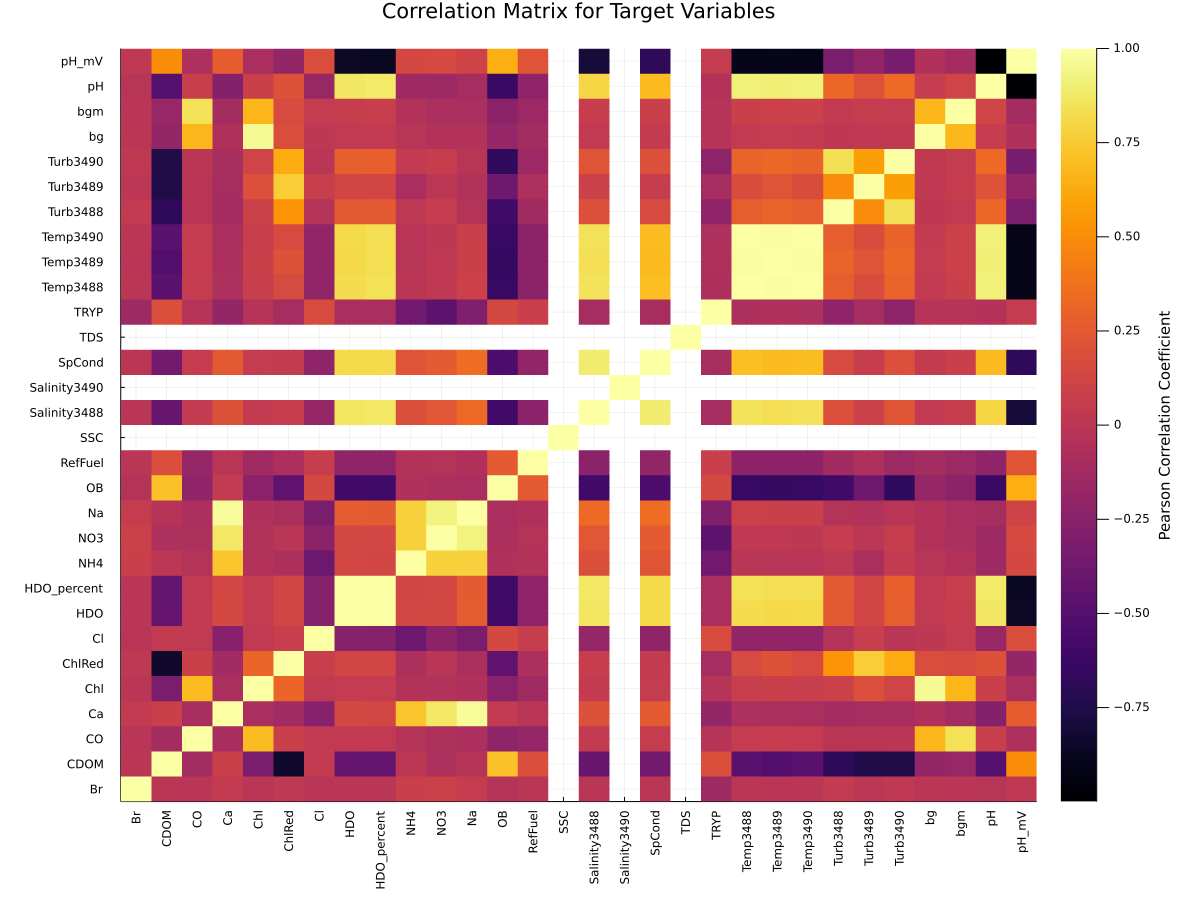
\includegraphics[width=0.85\columnwidth]{robot-team/supervised-2/correlation/target_cor.png}
\caption{Correlation Matrix for Target variables measured by the boat.\label{target_cor}}
\end{figure}

\begin{figure}[h]
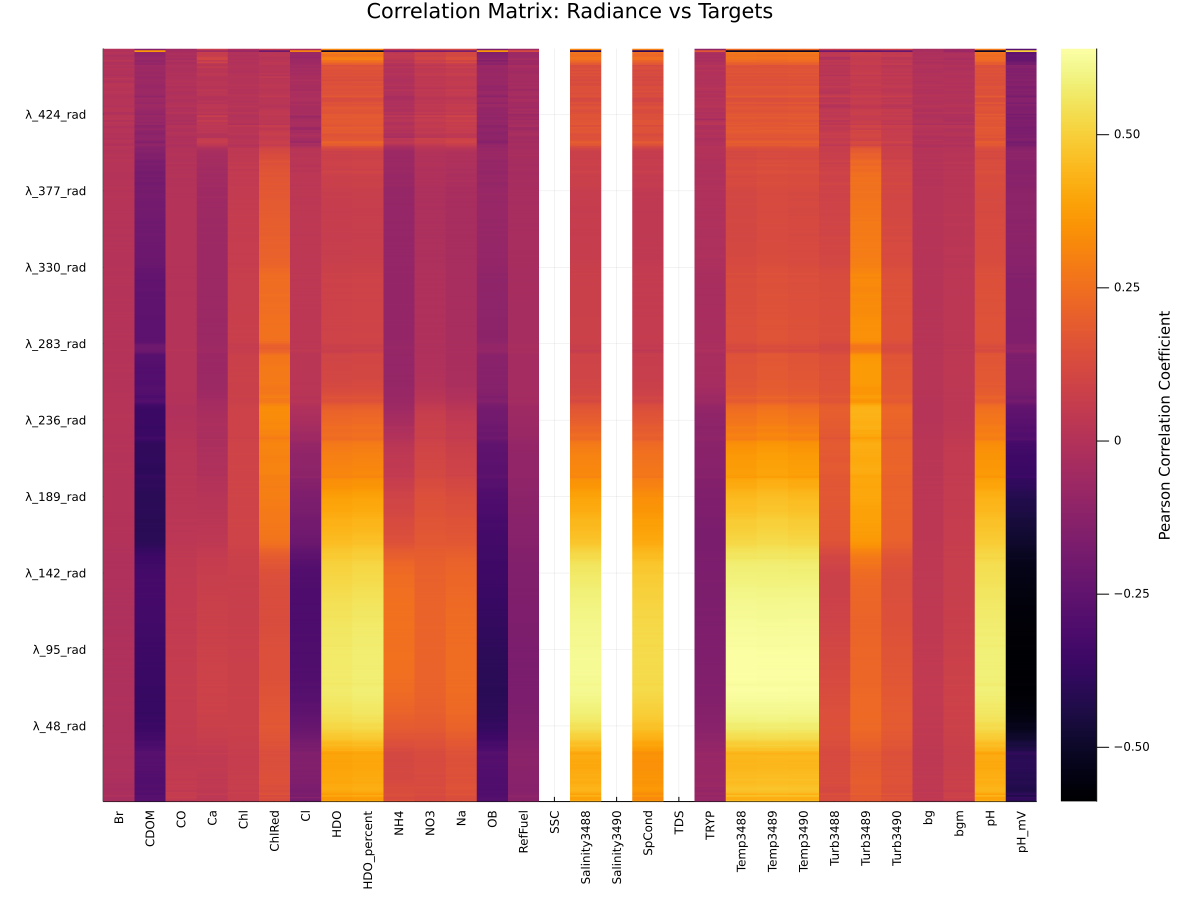
\includegraphics[width=0.85\columnwidth]{robot-team/supervised-2/correlation/radiance_cor.png}
\caption{Correlation Matrix for Radiance measurements versus Target Variables.\label{rad_cor}}
\end{figure}

\begin{figure}[h]
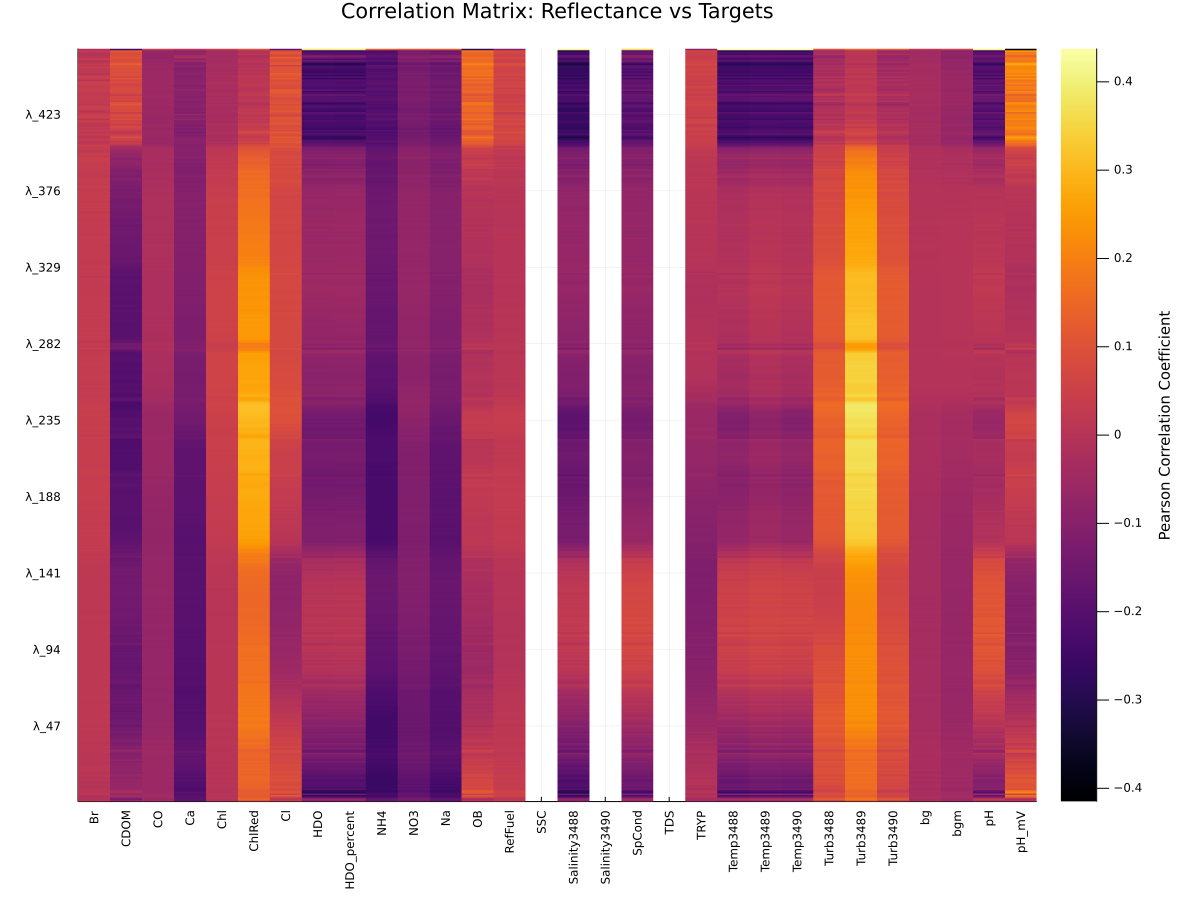
\includegraphics[width=0.85\columnwidth]{robot-team/supervised-2/correlation/reflectance_cor.png}
\caption{Correlation Matrix for Reflectance measurements versus Target Variables.\label{ref_cor}}
\end{figure}

\begin{figure}[h]
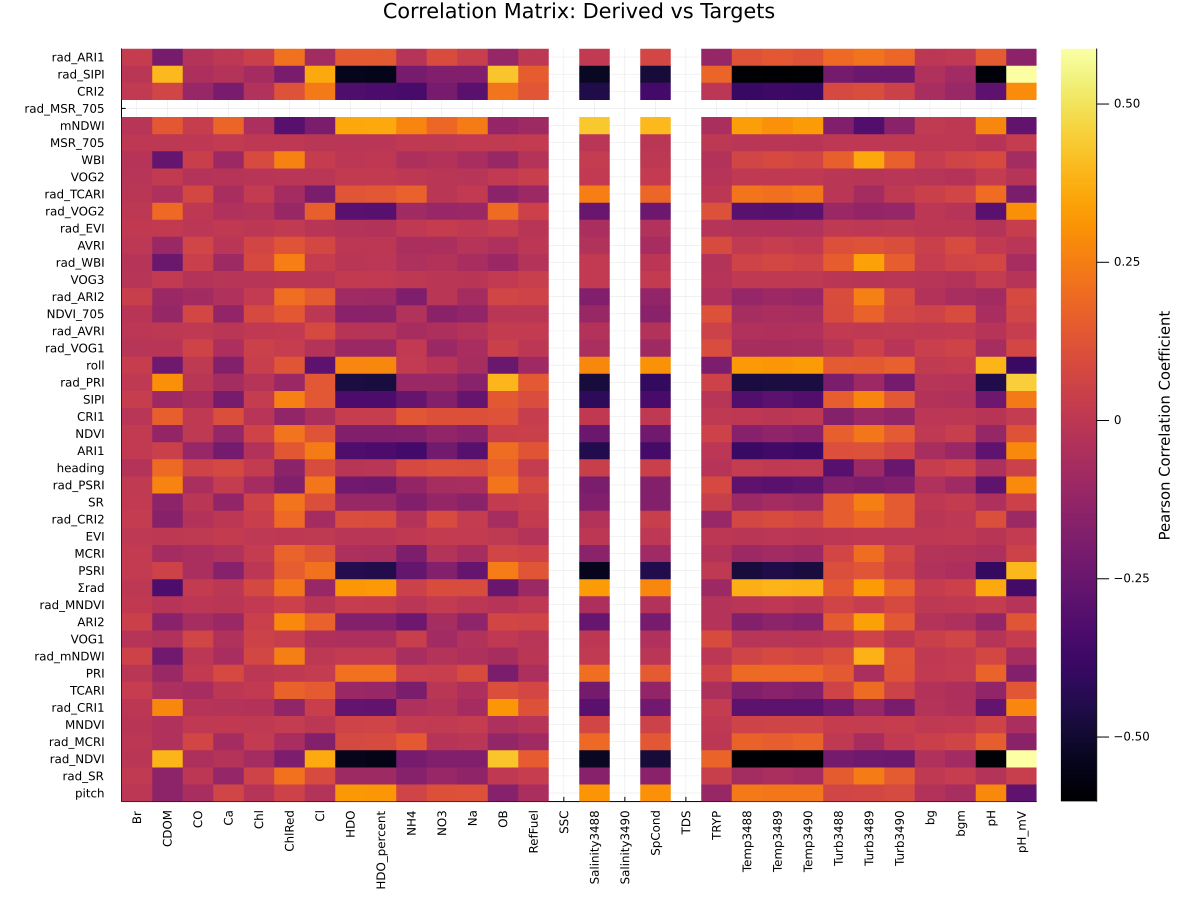
\includegraphics[width=0.85\columnwidth]{robot-team/supervised-2/correlation/derived_cor.png}
\caption{Correlation Matrix for derived measurements versus Target Variables.\label{derived_cor}}
\end{figure}



\subsubsection{Machine Learning Models}
include Linear Models, Neural Networks, Decision Trees, Bagging, Boosting, and Stacking\\

The field of Machine Learning has seen the invention of a plethora of models able to perform inference for regression tasks. Naturally, this leads to the challenge of evaluating which model is best for a given problem. In 1992 David Wolpert developed the notion of Stacked Generalization to divorce arbitrary human choice from the model selection process. [1] The key idea is as follows: fit an instance of each model compatible with your dataset. Each model learns different features of the data so that an adjudicating model (called the super-learner) can then be trained to map the predictions from each individual learner to a final output prediction. This is incredibly easy to accomplish in the Julia programming language via the MLJ machine learning framework [2]. We train a variety of learners including artificial neural networks, bagged decision trees, boosted decision trees, polynomial regressors, quantile regressors, LASSO regressors, and K-nearest-neighbors regressors. To ensure proper data hygiene, individual learners are first trained on separate cross validation folds so as not to bias the super-learner. After training the super-learner, each individual model is then trained on the full dataset to produce the best possible model.


paper on stacking \cite{ModelStacking}

\subsection{Model Analysis}
aleatoric and epistemic uncertainty

The black-box nature most machine learning methods makes it difficult to consider how errors propagate through a trained model during the inference process. For many problems such as image classification this is not an issue, however, in physical sensing error considerations are vital to establish detection limits and prediction confidence. Typically, there are three considerations we must make: measurement uncertainty– how much we can trust our model’s inputs, measurement representativeness– how well each data point represents data within a local neighborhood, and model error– how far the prediction is from the true value. Machine learning models are typically trained to minimize the model error. The Julia programming language makes it possible to handle all three. 


To address measurement uncertainty, we take advantage of Julia’s advanced automatic differentiation capabilities to enable differentiable programming (∂P). This means that we can take derivatives of our trained ML model with respect to each input feature to perform a sensitivity analysis. The final output uncertainty is then given via linear error propagation theory. [5]

Measurement representativeness can be trickier to handle. For example, in fluids it is common for two species to form a mixing layer that presents as a sharp discontinuity in measurement values. To quantify the degree to which neighboring points diverge we compute the average deviation across input measurements in a neighborhood around each data sample. This information can then be presented with model outputs to identify the regions where our model is valid. Similarly for ensemble ML models we compute the prediction deviation across all base learners to identify the representativeness of a data sample. Inputs that cause a large spread in base learner predictions indicate low representativeness in the training set. This analysis can then be used to plan further data collection missions that minimize time spent collecting data we have already present in our models. 

\subsubsection{Uncertainty Propagation via ($\partial P$)}

\subsubsection{Feature Ranking via SHAP values}

shape value paper used in ShapML.jl \cite{SHAPvalues1}

\subsubsection{Data Representativeness}
i.e. the average deviation across pixels used average during collocation process.
Also, we can look at relative disagreement between model predictions in bagged ensemble. 

\section{Results}
\subsection{CO}

\begin{figure}[h]
\includegraphics[width=0.85\columnwidth]{robot-team/supervised-2/CO/CO_dataMap.png}
\caption{Target distribution of CO at Scotty's Ranch.\label{CO_targetMap}}
\end{figure}

\begin{figure}[h]
\includegraphics[width=0.85\columnwidth]{robot-team/supervised-2/CO/CO_train-test_hist.png}
\caption{Stratified train-test split for CO.\label{CO_trainTestHist}}
\end{figure}

\begin{figure}[h]
  \begin{subfigure}{0.5\textwidth}
    \centering
    \includegraphics[width=0.95\linewidth]{robot-team/supervised-2/CO/rfr_CO_scatter.png}
  \end{subfigure}
  \begin{subfigure}{0.5\textwidth}
    \centering
    \includegraphics[width=0.95\linewidth]{robot-team/supervised-2/CO/rfr_CO_qq.png}
  \end{subfigure}
  \caption{(\textbf{a}) Scatterplot for the trained random forest Crudo Oil model. (\textbf{b}) Quantile-Quantile plot for the same fit.}
  \label{CO_fitresult}
\end{figure}



\begin{figure}[h]
    \includegraphics[width=0.85\columnwidth]{robot-team/supervised-2/CO/rfr_CO_featureImportance.png}
    \caption{Ranked feature importance for Crude Oil. Importance is determined via mean absolute SHAP value. \label{CO_shapely}}
\end{figure}






\section{Methods for Unsupervised Classification of Hyperspectral Scenes in Novel Environments}

\subsubsection{Unsupervised Classification}
\begin{figure}[h]
  \includegraphics[width=0.85\columnwidth]{robot-team/unsupervised/clustering.png}
  \caption{Unsupervised clustering of hyper-spectral image data using the K-means algorithm.\label{clustering}}
\end{figure}



